% DEFERRED CONTENT — NOT CURRENTLY COMPILED.
% This file holds the behavioural/dynamic layer of the notch model (Cobb--Douglas
% cost specification, marginal-buncher elasticity mapping, calibration-input and
% forward solution, and the reduced-form counterfactual density), moved verbatim
% out of Sections/model.tex. It is left for future work; it is not included in main.tex.

\subsection{A Cobb--Douglas cost specification}
\label{ssec:cost}

I specify cost through a one-input Cobb--Douglas technology relating turnover
$Y_i$ to input expenditure $X_i$,
\begin{equation}
  Y_i \;=\; A_i\, X_i^{\alpha},
  \qquad
  c_i(y_i) \;=\; \left(\frac{y_i}{A_i}\right)^{1/\alpha},
  \label{eq:production}
\end{equation}
where $A_i>0$ is a firm-specific cost/productivity parameter and $\alpha>0$ a
common returns-to-scale parameter. The implied marginal cost is
\begin{equation}
  \frac{\partial c_i(y_i)}{\partial y_i}
  \;=\; \frac{1}{\alpha}\,\frac{c_i(y_i)}{y_i}
  \;=\; \frac{1}{\alpha}\,\frac{X_i}{Y_i},
  \label{eq:mc}
\end{equation}
which a firm reveals through its input--output ratio in the data. The
returns-to-scale parameter is calibrated, in the companion calibration step, to
$\alpha \approx 0.989$, i.e.\ near-constant returns, so marginal cost is close to
$X_i/Y_i$.

I flag a degeneracy that this near-constant-returns value induces, and that the
implementing code makes explicit. The unconstrained interior optimum of
\eqref{eq:firm-problem} on either branch satisfies the first-order condition
$\mathrm{net} = \alpha^{-1} A_i^{-1/\alpha}\,y_i^{(1-\alpha)/\alpha}$, with
$\mathrm{net}=1$ below $T^{*}$ and $\mathrm{net}=1-\tau$ above, giving
\begin{equation}
  y_i^{\star} \;=\; A_i\,\bigl(\alpha\,\mathrm{net}\bigr)^{\alpha/(1-\alpha)}.
  \label{eq:interior}
\end{equation}
As $\alpha\to1$ the exponent $\alpha/(1-\alpha)\approx 90$ explodes, so the
taxed-branch optimum and the inversion of observed turnover back to productivity
become numerically ill-conditioned: tiny output differences map to enormous
differences in $A_i$. I therefore retain \eqref{eq:interior} and the
productivity inversion only as documented diagnostics, and base the behavioural
object below on the standard iso-elastic Kleven--Waseem representation rather
than on the Cobb--Douglas taxed-branch optimum. I am explicit about this because
it determines which equations are load-bearing: the dominated region of
Section~\ref{ssec:dominated} is \emph{exact} and survives the degeneracy, whereas
the Cobb--Douglas branch optimum does not.

\subsection{The marginal buncher and the elasticity mapping}
\label{ssec:buncher}

Firms whose frictionless optimum lies above $T^{*}$ choose between
\emph{bunching} at the threshold (remaining unregistered) and \emph{registering}
beyond the dominated region. The marginal buncher is the firm exactly indifferent
between the two; all firms with frictionless optimum in $(T^{*},\,y_H]$ bunch at
$T^{*}$, while firms above $y_H$ register and jump past the dominated region. The
width of the bunching segment $\Delta y^{*}=y_H-T^{*}$ is the structural
counterpart of the excess mass measured in Section~\ref{sec:bunching}, and it is
the bridge from that excess mass to a behavioural turnover elasticity.

\paragraph{The iso-elastic indifference condition.} Because
$\alpha\approx0.989$ renders the Cobb--Douglas taxed-branch optimum degenerate
(Section~\ref{ssec:cost}), I evaluate the marginal buncher in the standard
Kleven--Waseem iso-elastic representation \citep{klevenwaseem2013,saez2010},
in which a single behavioural elasticity $e$ governs the response. Index a firm
by its ability $n$, defined so that its frictionless (no-tax) optimum is exactly
$y=n$, and write its quasi-linear payoff with an iso-elastic cost of scaling
output as
\begin{equation}
  u(y;n) \;=\; \bigl(1-\tau\,\mathbb{1}\{y\ge T^{*}\}\bigr)\,y
  \;-\; \frac{n}{1+1/e}\left(\frac{y}{n}\right)^{1+1/e},
  \label{eq:isoelastic}
\end{equation}
where $e$ is the elasticity of turnover with respect to the net-of-tax rate.
A firm that registers chooses its interior optimum on the taxed branch,
\begin{equation}
  y_1(n) \;=\; n\,(1-\tau)^{e},
  \label{eq:postnotch-opt}
\end{equation}
obtained by maximising \eqref{eq:isoelastic} over the registered branch. The
marginal buncher is the ability level $n_H$ at which the firm is indifferent
between bunching at $T^{*}$ (paying no VAT, but constraining output) and
registering at $y_1(n_H)$. Writing $p \equiv 1+1/e$ and using that the
frictionless optimum of the marginal buncher equals its ability, $y_H=n_H$, the
indifference condition is
\begin{equation}
  \underbrace{T^{*} - \frac{n_H}{p}\left(\frac{T^{*}}{n_H}\right)^{\!p}}_{\text{bunch at }T^{*}}
  \;=\;
  \underbrace{(1-\tau)\,y_1(n_H) - \frac{n_H}{p}\left(\frac{y_1(n_H)}{n_H}\right)^{\!p}}_{\text{register at }y_1(n_H)},
  \qquad y_1(n_H)=n_H(1-\tau)^{e}.
  \label{eq:indiff}
\end{equation}
Equation~\eqref{eq:indiff} is the elasticity mapping. Given $e$ it has a unique
root $n_H>T^{*}$, solved numerically (a one-dimensional bracketed root-find on
the gap between the two sides), which delivers the marginal buncher
$y_H=n_H$ and hence the excess span $\Delta y^{*}=y_H-T^{*}$. Read in the other
direction, it is the structural inverse used in calibration: a measured
excess-mass span $\Delta y^{*}/T^{*}$ from the reduced-form bunching of
Section~\ref{sec:bunching} pins down the elasticity $e$ that reconciles it with
\eqref{eq:indiff}. This is the explicit form of the step that
Section~\ref{sec:bunching} described in prose as ``a separate structural step''
translating excess mass into a behavioural elasticity.

\paragraph{Calibrated values.} Evaluating \eqref{eq:indiff} at the elasticities
the companion calibration carries from the bunching evidence gives
$y_H=\pounds127{,}382$ (so $\Delta y^{*}=\pounds42{,}382$ and
$\Delta y^{*}/T^{*}=0.50$) at the median elasticity $e=0.17$, rising to
$y_H=\pounds143{,}527$ ($\Delta y^{*}=\pounds58{,}527$) at the mean elasticity
$e=0.32$. In both cases $y_H$ lies well above the dominated region, as it must:
the marginal buncher registers strictly beyond $T^{*}+a=\pounds106{,}250$.
Figure~\ref{fig:notch-fit} places these structural objects against the observed
turnover distribution: the empty dominated region of width $a=\pounds21{,}250$
above the threshold and the marginal buncher at $y_H=\pounds127{,}382$. The
frictionless model would relocate every firm with a frictionless optimum below
$y_H$ to a single spike at $T^{*}$---a mass orders of magnitude larger than the
observed excess bunching. That spike is not what the data show: the gap between
it and the modest observed bunching is precisely optimisation friction, and the
observed mass that remains \emph{inside} the dominated region is a direct reading
of that friction.

\begin{figure}[t]
  \centering
  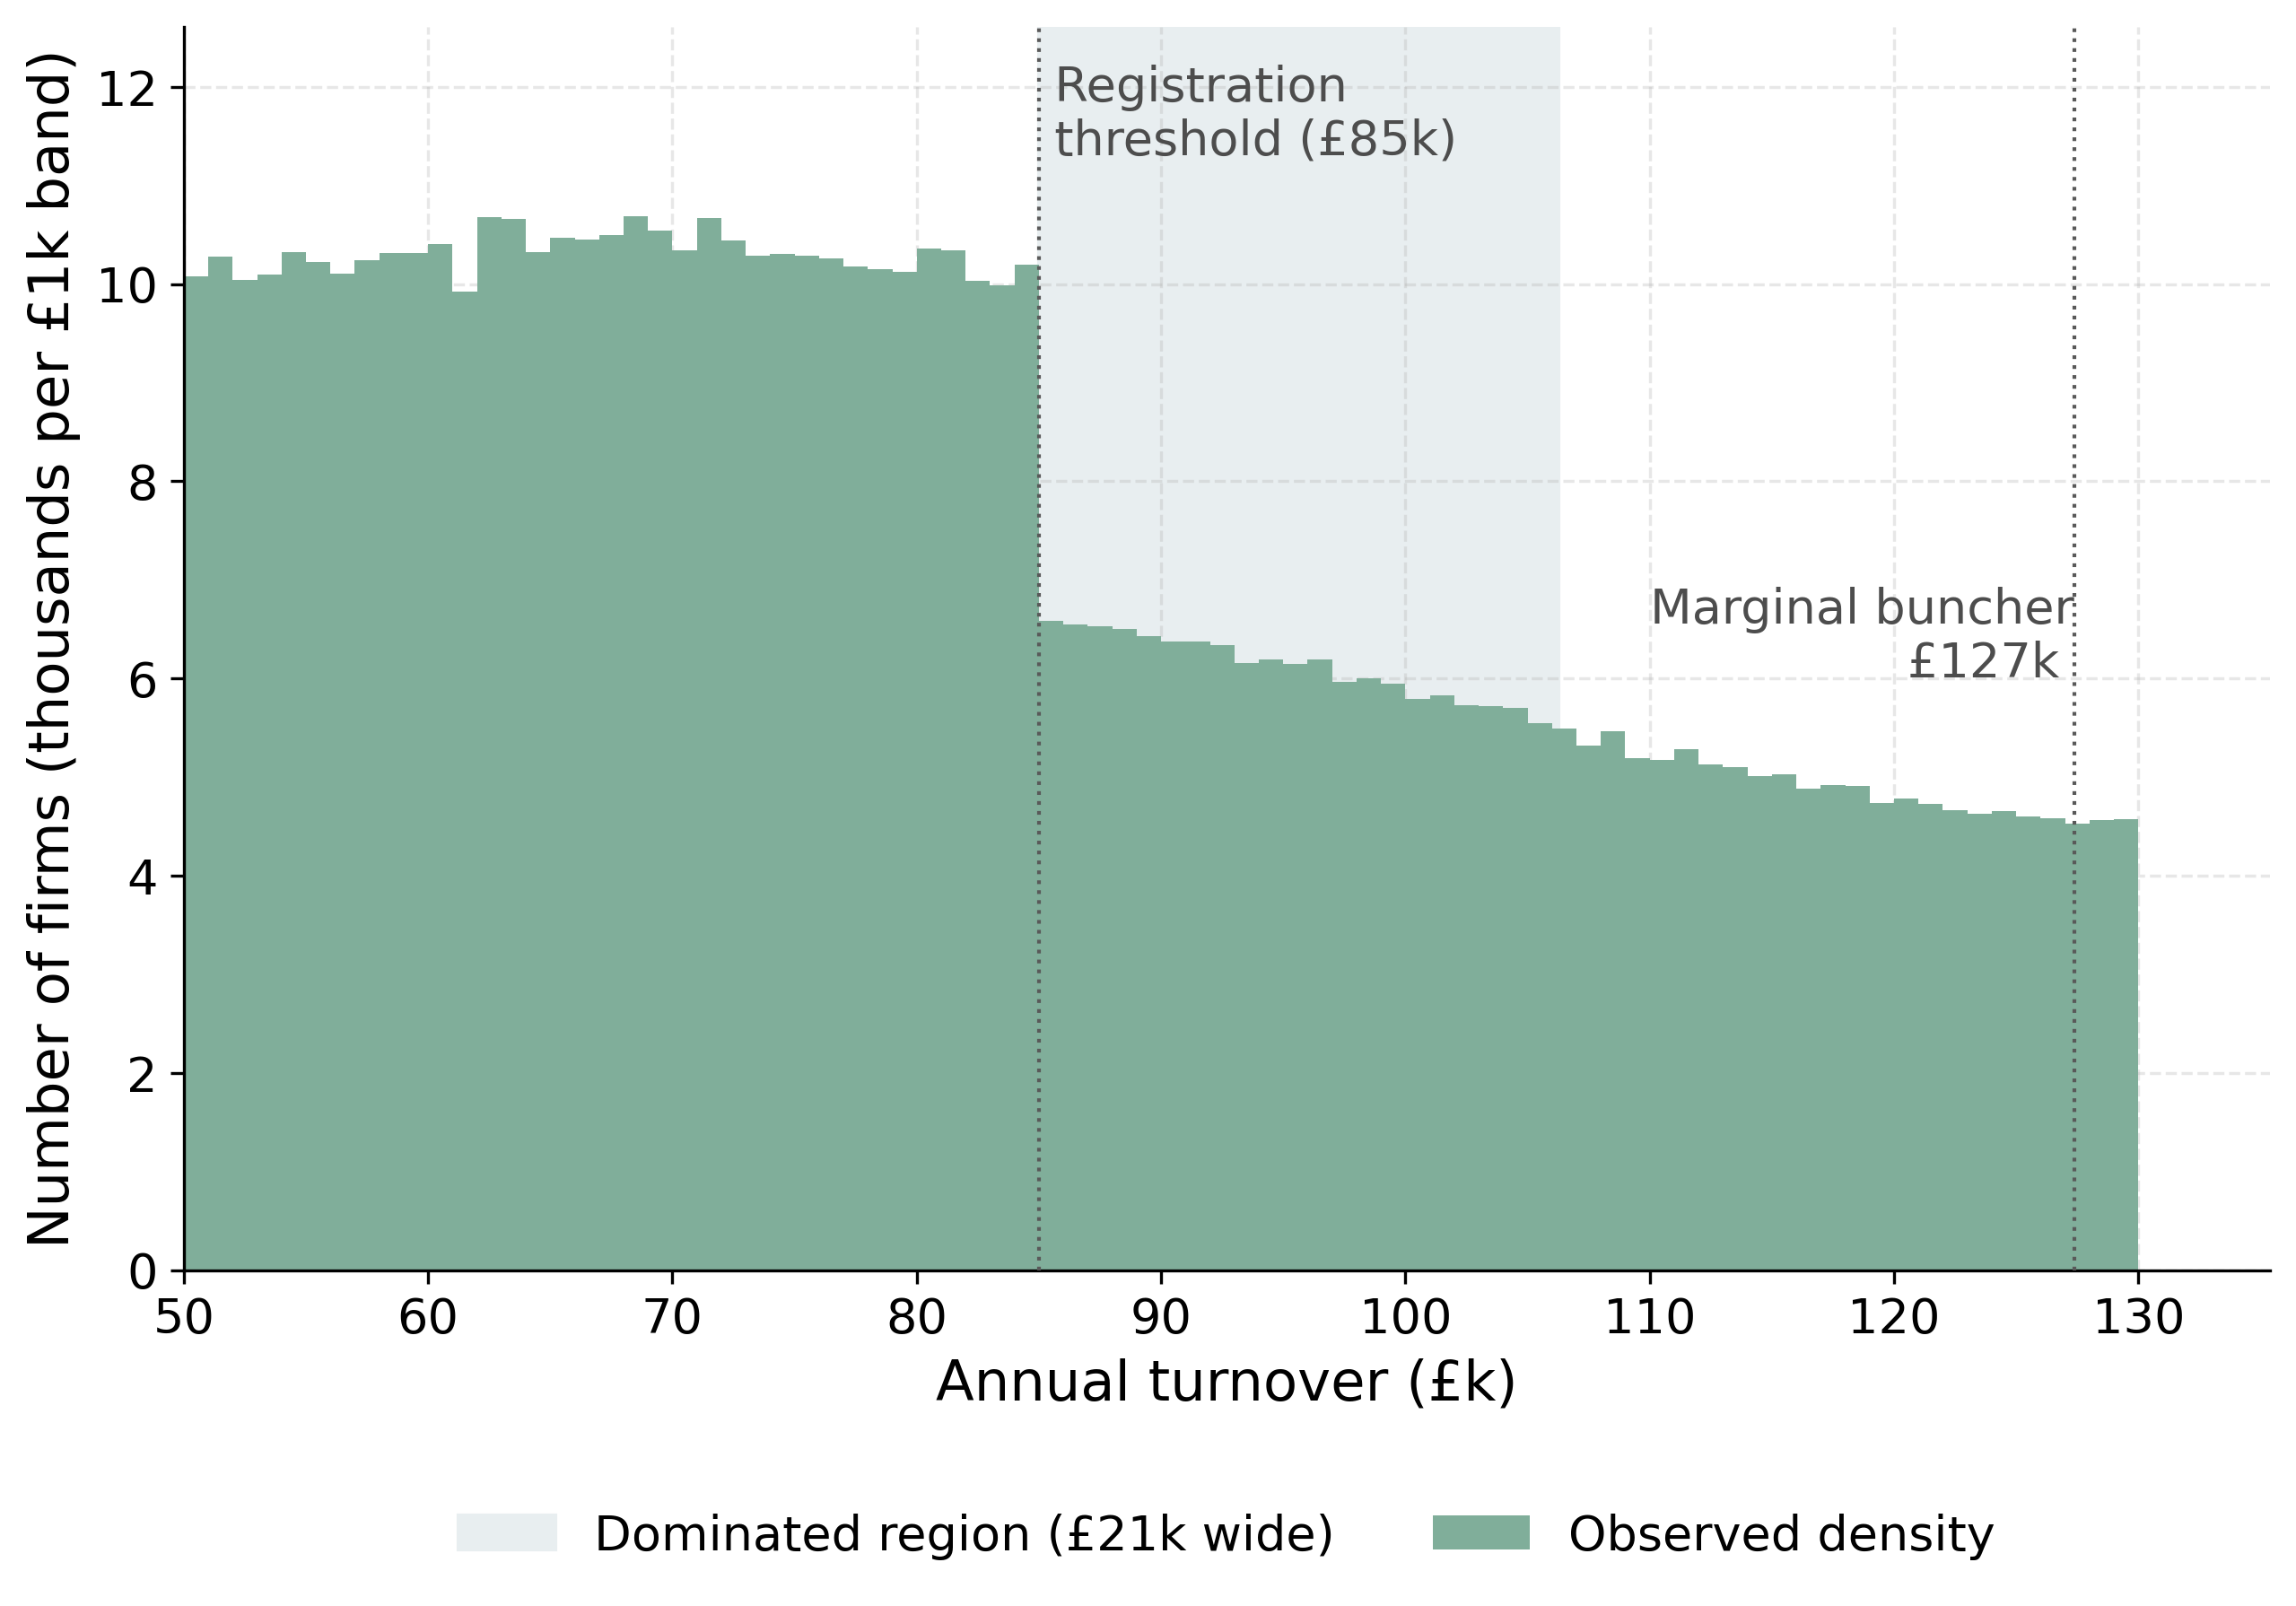
\includegraphics[width=0.85\textwidth]{figures/notch_model_fit.png}
  \caption{Mechanism of the VAT notch at $T^{*}=\pounds85{,}000$, shown at the
    observed scale. The structural objects---the empty dominated region of width
    $a=\pounds21{,}250$ (shaded) and the marginal buncher $y_H=\pounds127{,}382$
    (at the median turnover elasticity $e=0.17$)---are overlaid on the observed
    synthetic turnover density. Frictionlessly the notch would send every firm
    below $y_H$ to a spike at $T^{*}$ orders of magnitude above the observed
    bunching; that spike is omitted as uninformative, and the observed mass
    remaining inside the dominated region measures the optimisation frictions
    that attenuate the response.}
  \label{fig:notch-fit}
\end{figure}

\subsection{The calibration input and forward solution}
\label{ssec:recovery}

To re-solve the firm's problem under a counterfactual schedule I need a
firm-level cost parameter consistent with each firm's observed allocation. I
take it as the production residual implied by \eqref{eq:production},
\begin{equation}
  A_i \;=\; \frac{Y_i}{X_i^{\alpha}},
  \label{eq:recover}
\end{equation}
using only observed turnover $Y_i$, inputs $X_i$, and the calibrated $\alpha$.
This residual is a \emph{calibration input}, not an identified structural
primitive: it is whatever cost level rationalises the firm's observed turnover
and inputs at the $\pounds85{,}000$ schedule, and I hold it fixed when I change
the schedule. I make no claim that $\{A_i\}$ is policy-invariant or recovers a
structural productivity distribution---the contribution of
\citet{garicano2016} and \citet{gourioroys2014}---only that it is a fixed
accounting anchor for a forward simulation.

\paragraph{Forward solution.} Holding $\{A_i\}$ fixed, I re-solve each firm's
problem with the schedule replaced by a counterfactual---a relocated threshold, a
changed rate, or a tapered schedule. For this computation I represent the
schedule with a smooth (sigmoid) effective rate,
\begin{equation}
  \tau(y) \;=\; \frac{\tau}{1+e^{-k(y-T^{*})}},
  \label{eq:tau-smooth}
\end{equation}
whose steepness $k$ is calibrated so that the smooth schedule reproduces the
dominated region of Section~\ref{ssec:dominated}; the equivalence of this smooth
representation to the exact notch is the subject of a separate robustness
appendix. Because the near-constant-returns technology makes a differentiable
first-order condition ill-conditioned (Section~\ref{ssec:cost}), I locate each
firm's optimum by maximising after-tax profit directly over a bounded grid
around its observed turnover rather than by root-finding on \eqref{eq:interior}.
The bounded window is a modelling assumption, justified by the localisation of
the realised response; I flag that it mechanically limits how far firms
reposition. The smooth schedule \eqref{eq:tau-smooth} and the grid search are the
\emph{computational implementation} of the notch model, not a competing
specification. A change to the \emph{shape} of the schedule has no single point of
excess mass to forward-map, so the reduced-form counterfactual of
Section~\ref{sec:bunching} is silent on it. The robust, headline statement about
such reforms is therefore the analytic one above---how each alters the dominated
region (Section~\ref{ssec:dominated})---which, together with the static revenue
costs of Section~\ref{ssec:schedule_costs}, characterises the reforms without
relying on the parameter-sensitive re-optimised magnitudes. The forward solution
\eqref{eq:tau-smooth} is the computational tool behind these objects; it is
distinct from the reduced-form density counterfactual described next.

\subsection{A reduced-form counterfactual density}
\label{ssec:cf-density}

To quantify the distortion induced by the notch I also require the turnover
distribution that would obtain in its absence. Rather than re-solving the firm's
problem, this object estimates the smooth, undistorted size distribution directly
from the data, using the same polynomial counterfactual as the reduced-form
bunching estimator of Section~\ref{sec:bunching}. Measuring each observation by
its distance from the cutoff $y_{\mathrm{dist}} = T - T^{*}$, I fit a third-order
polynomial by ordinary least squares to the data outside a window
$[\,T^{*}-W,\; T^{*}+W\,]$ with $W=\pounds15{,}000$,
\begin{equation}
  f^{\mathrm{cf}}(T) \;=\;
  \beta_0 + \beta_1\, y_{\mathrm{dist}} + \beta_2\, y_{\mathrm{dist}}^{2}
  + \beta_3\, y_{\mathrm{dist}}^{3},
  \label{eq:cf-poly}
\end{equation}
and project it back into the excluded region. The gap between the observed density
and~\eqref{eq:cf-poly}---excess mass below $T^{*}$ and missing mass above
it---measures the behavioural response, in the reduced-form tradition of
\citet{liuetal2021}; it is not the structural re-optimisation that the forward
solution of Section~\ref{ssec:recovery} performs.
